%% This is file `elsarticle-template-1-num.tex',
%%
%% Copyright 2009 Elsevier Ltd
%%
%% This file is part of the 'Elsarticle Bundle'.
%% ---------------------------------------------
%%
%% It may be distributed under the conditions of the LaTeX Project Public
%% License, either version 1.2 of this license or (at your option) any
%% later version.  The latest version of this license is in
%%    http://www.latex-project.org/lppl.txt
%% and version 1.2 or later is part of all distributions of LaTeX
%% version 1999/12/01 or later.
%%
%% The list of all files belonging to the 'Elsarticle Bundle' is
%% given in the file `manifest.txt'.
%%
%% Template article for Elsevier's document class `elsarticle'
%% with numbered style bibliographic references
%%
%% $Id: elsarticle-template-1-num.tex 149 2009-10-08 05:01:15Z rishi $
%% $URL: http://lenova.river-valley.com/svn/elsbst/trunk/elsarticle-template-1-num.tex $
%%
\documentclass[preprint,12pt]{elsarticle}
\usepackage{amsmath}
\usepackage{graphicx,subcaption}
\usepackage{listings}
\usepackage{hyperref}
\usepackage{multirow}
\usepackage{notoccite}
\hypersetup{
    colorlinks,
    citecolor=black,
    filecolor=black,
    linkcolor=black,
    urlcolor=black
}

%% Use the option review to obtain double line spacing
%% \documentclass[preprint,review,12pt]{elsarticle}

%% Use the options 1p,twocolumn; 3p; 3p,twocolumn; 5p; or 5p,twocolumn
%% for a journal layout:
%% \documentclass[final,1p,times]{elsarticle}
%% \documentclass[final,1p,times,twocolumn]{elsarticle}
%% \documentclass[final,3p,times]{elsarticle}
%% \documentclass[final,3p,times,twocolumn]{elsarticle}
%% \documentclass[final,5p,times]{elsarticle}
%% \documentclass[final,5p,times,twocolumn]{elsarticle}

%% if you use PostScript figures in your article
%% use the graphics package for simple commands
%% \usepackage{graphics}
%% or use the graphicx package for more complicated commands
%% \usepackage{graphicx}
%% or use the epsfig package if you prefer to use the old commands
%% \usepackage{epsfig}

%% The amssymb package provides various useful mathematical symbols
\usepackage{amssymb}
%% The amsthm package provides extended theorem environments
%% \usepackage{amsthm}

%% The lineno packages adds line numbers. Start line numbering with
%% \begin{linenumbers}, end it with \end{linenumbers}. Or switch it on
%% for the whole article with \linenumbers after \end{frontmatter}.
\usepackage{lineno}

%% natbib.sty is loaded by default. However, natbib options can be
%% provided with \biboptions{...} command. Following options are
%% valid:

%%   round  -  round parentheses are used (default)
%%   square -  square brackets are used   [option]
%%   curly  -  curly braces are used      {option}
%%   angle  -  angle brackets are used    <option>
%%   semicolon  -  multiple citations separated by semi-colon
%%   colon  - same as semicolon, an earlier confusion
%%   comma  -  separated by comma
%%   numbers-  selects numerical citations
%%   super  -  numerical citations as superscripts
%%   sort   -  sorts multiple citations according to order in ref. list
%%   sort&compress   -  like sort, but also compresses numerical citations
%%   compress - compresses without sorting
%%
%% \biboptions{comma,round}

% \biboptions{}

\let\originaleqref\eqref
\renewcommand{\eqref}{Eq.~\originaleqref}

\hypersetup{colorlinks=true,
  pdftitle={Performance and Accuracy of WARP - A Framework for Continuous Energy Monte Carlo Neutron Transport in General 3D Geometries on GPUs},
  pdfauthor={Ryan M. Bergmann, Kelly Rowland, Nikola Radnovi\'c, Rachel Slaybaugh?, Jasmina L. Vuji\'c}}

\journal{Annals of Nuclear Energy}

\begin{document}

\begin{frontmatter}

%% Title, authors and addresses

%% use the tnoteref command within \title for footnotes;
%% use the tnotetext command for the associated footnote;
%% use the fnref command within \author or \address for footnotes;
%% use the fntext command for the associated footnote;
%% use the corref command within \author for corresponding author footnotes;
%% use the cortext command for the associated footnote;
%% use the ead command for the email address,
%% and the form \ead[url] for the home page:
%%
%% \title{Title\tnoteref{label1}}
%% \tnotetext[label1]{}
%% \author{Name\corref{cor1}\fnref{label2}}
%% \ead{email address}
%% \ead[url]{home page}
%% \fntext[label2]{}
%% \cortext[cor1]{}
%% \address{Address\fnref{label3}}
%% \fntext[label3]{}

\title{Performance and Accuracy of WARP - A Framework for Continuous Energy Monte Carlo Neutron Transport in General 3D Geometries on GPUs}

%% use optional labels to link authors explicitly to addresses:
%% \author[label1,label2]{<author name>}
%% \address[label1]{<address>}
%% \address[label2]{<address>}

\author{Ryan M. Bergmann \corref{rmb}}
\ead{ryanmbergmann@gmail.com}
\cortext[rmb]{Corresponding author. Tel.: +41.76.687.53.09.}

\author{Kelly Rowland }
\ead{krowland@berkeley.edu}

\author{Nikola Radnovi\'c }
\ead{radnovicn@gmail.com}

\author{Rachel Slaybaugh?}
\ead{slaybaugh@berkeley.edu}

\author{Jasmina L. Vuji\'c }
\ead{vujic@nuc.berkeley.edu}


\address{Department of Nuclear Engineering, 
4155 Etcheverry Hall, 
University of California - Berkeley,
Berkeley, CA 94703-1730}

\begin{abstract}

In this companion paper to ``Algorithmic Choices in WARP - A Framework for Continuous Energy Monte Carlo Neutron Transport in General 3D Geometries on GPUs'' (doi:10.1016/j.anucene.2014.10.039), the WARP Monte Carlo neutron transport framework for GPUs is benchmarked against production-level CPU Monte Carlo neutron transport codes for both performance and accuracy.  Fission source distributions, flux spectra, and multiplication factors calculated by WARP are compared to those from Serpent v2.XX.X and MCNP v6.1. for identical materials and geometries.  Runtimes are also reported.

\end{abstract}

\begin{keyword}
Monte Carlo \sep Neutron Transport \sep GPU \sep CUDA \sep CUDPP \sep OptiX


\end{keyword}

\end{frontmatter}

\linenumbers

%% main text

\section{Introduction}
\label{sec:intro}

Developing WARP was motivated by modern supercomputers commonly being built with graphics processing units (GPU) coprocessor cards in their nodes to increase their computational efficiency and performance \cite{}.  Compared to more common central processing units, or CPUs, GPUs have a larger aggregate memory bandwidth, much larger rate of floating-point operations per second (FLOPS), and lower energy consumption per FLOP\cite{}.  GPUs execute efficiently on data-parallel problems \cite{}, and since most CPU codes are task-parallel, the algorithms used had to be reconsidered.  Data-parallelism is simply parallelism that arises from operating on many different pieces of data at one time, whereas task-parallelism is parallelism that arises from running many concurrent tasks at one time which act on a single piece of data.   Figure \ref{datavtask} shows and illustration of the difference between a data-parallel and a task-parallel neutron transport loop.

\begin{figure}[h!] 
  \centering
    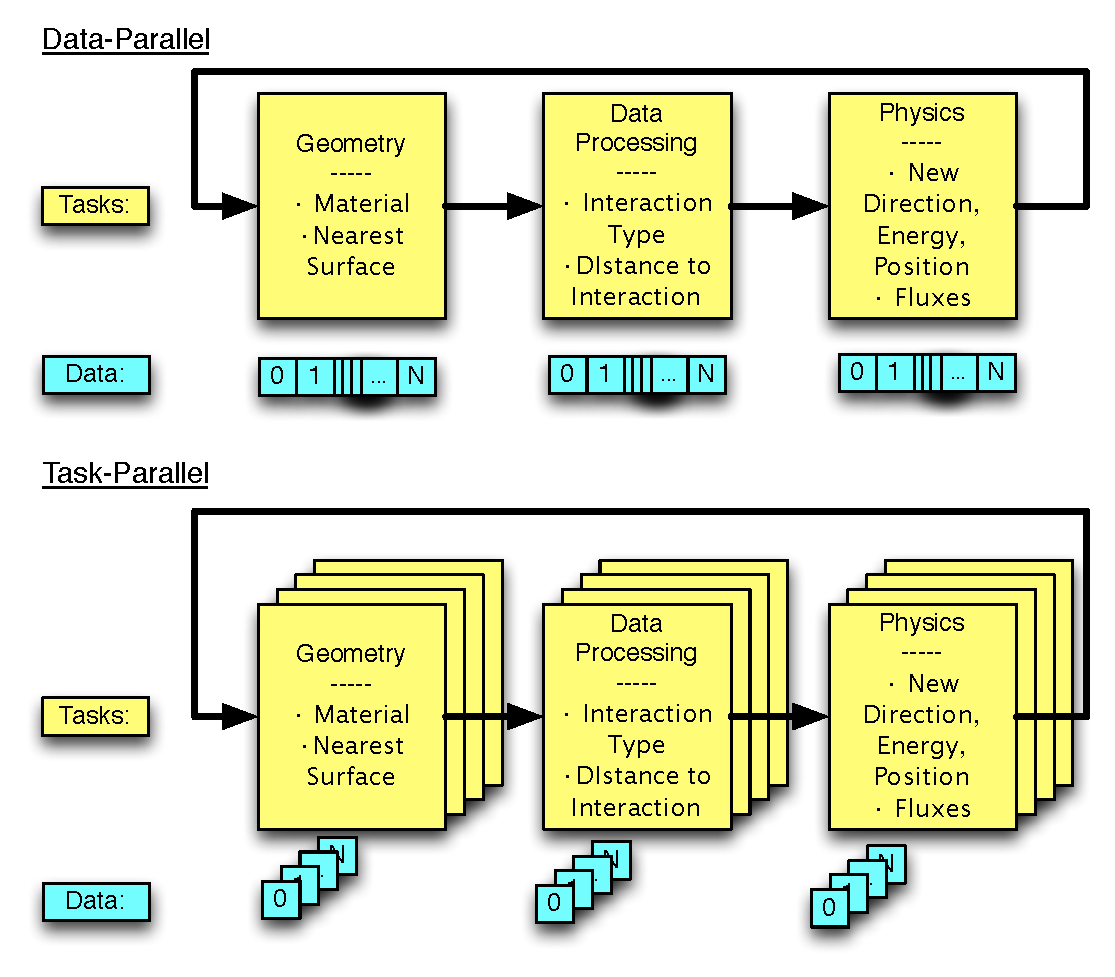
\includegraphics[width=\textwidth]{graphics/datavtask.pdf}
     \caption{Data-parallel neutron trasport loop vs. a task-parallel transport loop for N neutrons in parallel.  \label{datavtask} }
\end{figure}

Execution on GPUs also requires additional data management, since the on-chip memory of the GPU is separate from the host CPUs memory \cite{cuda}.  Execution on NVIDIA GPUs also required code to be written in CUDA, which is a set of extensions for C/C++.  The simplest way to accommodate all these requirements was to write a new code from scratch, which ultimately resulted in WARP.  

In this paper, results calculated by WARP are compared against those calculated by Serpent 2.XX.X and MCNP 6.1, two widely-used production-level Monte Carlo neutron transport codes, in order to ensure the accuracy of WARP and to highlight its performance differences.  The details about the algorithms used in WARP are discussed in \cite{algorithms}.


%%%%%%%%%%%%%%%%%%%
%%%%%%%%%%%%%%%%%%%
%%%%%%%%%%%%%%%%%%%
\section{Features of WARP}
\label{sec:features}

WARP has only existed since 2013, and is not as fully-featured as more mature Monte Carlo codes.  It has the functionality necessary to compare its performance against  Serpent 2.XX.X and MCNP 6.1, and this section outlines the current set of features available in WARP.  

\subsection{Physics}

Only neutrons are transported by WARP.  Any other particles are not considered in any way.  WARP loads ACE-formatted nuclear data libraries via the ``ace'' module in PyNE \cite{}.  The cross section data are then re-formatted to use a unionionzed energy grid via numpy, then then passed to the C++ routines via the Python C API.  Cross section data compiled by the United States is distributed by the Department of Energy in \emph{ENDF} files.  ENDF stands for ``evaluated nuclear data file,'' and can contain data for nuclear decay, photons, atomic relaxation, fission yields, thermal neutron scattering, and charged particle reactions as well as neutron reactions.  ACE stands for ``a compact ENDF'' and strips out a lot of the extra information unnecessary for neutron transport.  Since many Monte Carlo codes read ACE-formatted data rather than the original ENDF file, WARP can eliminate one potential cause for discrepancies by loading identical data as other codes.  

In its current state, WARP does not use the thermal scattering (S($\alpha,$$\beta$)) tables or unresolved resonance parameters and only uses the free-gas approximation for target nuclei.  This treats the target as part of a gas at a certain temperature and does not consider anything other than purely elastic scattering. Thermal scattering and unresolved resonance data tables improve the physical fidelity of the simulation, but these features can be turned off in production codes and direct comparisons can be made without them.  Their incorporation may lead to more divergent program flow and is left as an area of future work.

WARP currently also only has a handful of the most common ENDF sampling laws implemented.   These are laws 2, 3, 44,and XXX \cite{MCNP}.  Some nuclei have interactions that require the remaining laws (XXX), and therefore problems containing any such nuclides cannot be solved.

\subsection{Geometry}

The geometry representation in WARP is handled by the NVIDIA OptiX library, which provides high performance on the GPU, but imposes some limitations on the how geometries must be input.

\begin{enumerate}
\item Cells are the basic building blocks, not surfaces, and all cells must be finite and closed.
\item Implicit nesting determines what material exists inside of a cell.  In other words, since cells are defined directly, the material of cell A is only that space where cell A is the lowest nested cell.  If cell B is within cell A, the entire space within cell B is excluded from cell A simply because cell B resides within cell A and does not need to be excluded explicitly.
\item The only cell types available are spheres, cylinders, right rectangular prisms, and right hexagonal prisms.
\item Only translational transforms have been implemented, although this restriction could be lifted by some additional development.
\end{enumerate}

\subsection{Features}

WARP is mainly written in C/C++ and is compiled to a shared library.   and  with Python.  Pythonic wrapping is done via SWIG \cite{swig}, which automatically wraps compiled languages like C/C++ in high-level scripting languages.  With the C++ classes exposed in Python, the main() function can be replaced with a Python script, eliminating the need recompiled a main function and link it to the WARP library when different geometries or different run parameters are desired.  Of course, there is flexibility as well, and one could write a main function that could handle all conceivable cases. 

The Python wrapping approach deviates from the standard flat text input file structure that many Monte Carlo codes use.  Flat text input relies on keywords and adds a layer where input files need to be parsed and data structures are then built in the application based on the information parsed from the input.  Using Python to directly access the classes and their data removes this layer, and allows a user to build complex, custom applications if necessary.  Since the results would also be resident in a Python session and would therefore be easily available to the user for potting scripts or analysis tools.  To process data in the same way from text-file-based output, the output needs to be parsed with a user written function or processed by hand, which is time consuming and can lead to human error.

single volume tally
only collision estimators
no importance, variance reduction, or other convergence estimation beyond relative error


%%%%%%%%%%%%%%%%%%%
%%%%%%%%%%%%%%%%%%%
%%%%%%%%%%%%%%%%%%%
\section{Tests}
\label{sec:tests}

CPU/GPU hardware 

why running with 1e5 per batch, and 1e6, push titan to limit!

\subsection{Test 1}

table of isotopes, densities, dimensions for all tests

jezebel

\subsection{Test 2}

pin cell

\subsection{Test 3}

hom. pebble in flibe?

\subsection{Test 4}

sodium with SS clad over metallic fuel?

\subsection{Test 5}

assembly w clad in water


\subsection{Test 6}

fixed source, fusion 14.1 mev neutrons in shells of lithium and SiC and steel?  flux in sic first wall

\subsection{Test 7}

fixed source,  plane source at end of steel tube, u fission multiplier, flux in volume after u



%%%%%%%%%%%%%%%%%%%
%%%%%%%%%%%%%%%%%%%
%%%%%%%%%%%%%%%%%%%
\section{Results}
\label{sec:results}

\subsection{Test 1}
\subsection{Test 2}
\subsection{Test 3}
\subsection{Test 4}
\subsection{Test 5}
\subsection{Test 6}
\subsection{Test 7}

\subsection{Summary}

table of keff, 1-norm of rel err, 1-norm of some sort of fission distribution




%%%%%%%%%%%%%%%%%%%
%%%%%%%%%%%%%%%%%%%
%%%%%%%%%%%%%%%%%%%
\section{Conclusions and Future Development}
\label{sec:conc}

%WARP has shown that GPUs are an effective platform for performing Monte Carlo neutron transport with continuous energy cross sections.  Currently, WARP is the most detailed and feature-rich program in existence for performing continuous energy Monte Carlo neutron transport in general 3D geometries on GPUs, but compared to production codes like Serpent and MCNP, WARP has limited capabilities.  Despite WARP's lack of features, its novel algorithm implementations show that high performance can be achieved on a GPU despite the inherently divergent program flow and sparse data access patterns.  %WARP is not ready for everyday nuclear reactor calculations, but is a good platform for further development of GPU-accelerated Monte Carlo neutron transport.  In it's current state, it may be a useful tool for multiplication factor searches, i.e. determining reactivity coefficients by perturbing material densities or temperatures, since these types of calculations typically do not require many flux tallies. 
%Remapping threads to active data is an effective way of raising the processing rate when the number of active neutrons becomes small; this also reduces thread divergence in reaction kernels.  Using a radix sort to do the remapping is effective since it segregates reactions into contiguous blocks, efficient since it can be done in place and in $O(kN)$ time, and can eliminate completed data from being accessed if slight modifications to the standard reaction number encodings are made.  



there are many areas where feature need to be added in order for WARP to become a useful engineering and scientific tool - sab, unres, tallies, less intense memory layout (fractional cascade? grid thinning? on the fly temp would help a lot here too!), more geom types, meshes
Track length tallies would be very easy to implement
Will be released at open source software, pending DOE approval.

The development of WARP has led to important conclusions regarding how to conduct neutron transport on GPUs.  The first is that running with large datasets, and therefore a large number of threads, is important for good performance.  It was found that in some cases, moving from $10^5$ to $10^6$ neutrons per batch in criticality mode increase performance by a factor of four or more.  It is important to keep the GPU saturated with threads so it can effectively pipeline data loads.  

The initial goals of WARP have been completed, but there is much work still to be done if it is going to be of real use to the nuclear engineering community.  Basic functionality is currently good enough to assure the GPUs can accelerate high-fidelity Monte Carlo neutron transport calculations, which was the point of this work, but many capabilities need to be expanded and ensured to scale well to large numbers of neutrons, isotopes, and geometrical zones.

The geometry is currently handled by OptiX since it provides a convenient way to obtain high-performance results, but its execution had to be coerced into providing WARP with the information it needed, namely the material number via the point-in-polygon algorithm.  The way OptiX executes this algorithm is not efficient since it must be done iteratively using OptiX's native functions instead of calculating the ordered list of intersections in a single trace.  NVIDIA is releasing ``OptiX Prime'' with OptiX 3.5 \cite{optix3.5}, which promises to provide a more ``to the metal'' ray tracing experience, and might be leveraged to provide more efficient single-traverse functionality.  OptiX could also be replaced by Rayforce \cite{rayforce}, a high-performance GPU ray tracing library developed by VSL that has this functionality built-in and is currently available free of charge for noncommercial use.

The geometry routines could also be replaced by handwritten routines that use combinatorial solid geometry like Serpent and MCNP.  This would make writing input for WARP more like what most nuclear engineers are already used to and, more importantly, could provide a potential performance increase.  A universe-based CSG representation may map very well to the GPU and may even be able to fit inside of shared memory for small numbers of surfaces.  The surfaces may also be able to be bound to texture memory, which could provide a performance boost since it automatically caches for spatial locality.  

Using an efficient CSG method would further lend itself to using Woodcock delta-tracking for the neutrons and thus getting rid of the tracing algorithms and libraries altogether.  These algorithms account for about 50\% of execution time, and WARP's performance could be doubled by making the geometry routines more efficient.  If OptiX is determined to be the best option out of these others, however, a routine would need to be developed to automatically space coincident surfaces appropriately without specific user input.

WARP's execution can also be improved.  The amount of memory required per neutron was not tracked in this initial development, much less optimized, since developing a functioning code was the main priority.  Reducing the memory needed per neutron would be highly beneficial in the sense that more concurrent neutrons could be launched using the reclaimed memory space.  Dynamic parallelism can be implemented to minimize kernel launch overhead and host-device communication in the inner transport loop.  Dynamic parallelism is a feature introduced into the NVIDA Kepler GPUs that allows kernels to be launched from kernels, and could eliminate the host needing to contain the main transport loop.  Neither CUDPP or OptiX support its use, however.  CUDPP could be replaced with newer, higher-performance libraries (e.g.\ CUB) that do support dynamic parallelism, but OptiX would have to be replaced by a handwritten kernel to perform the necessary geometric tasks.  Textures could be thoroughly investigated as they might provide better performance in tasks where their free linear interpolation and spatial caching could provide a performance boost, like in an energy grid search on a tree structure.   Alternatively, using optimized graph search libraries, such as ``gunrock,'' could be used to perform the energy grid search.

WARP also currently only supports fixed-source mode in the non-remapping version as it requires popping secondary neutrons back into the active neutron pool after every iteration of the inner transport loop.  This operation is expensive since it is a global operation that must be done often.  This algorithm could be changed to be more like a criticality run, where the primary neutrons are all transported together, then the next (smaller) generation of secondary particles are transported, then the next, and so on.  This way, the pop routine is only executed in the outer loop, and could produce faster results.  Multi-GPU support should also be added so that WARP can be used effectively on computers with more than a one GPU.

If an entire overhaul of the WARP transport algorithm is feasible, using a SM-based algorithm might be investigated instead of current global one.  This type of algorithm would treat each SM as an independent processor, and would provide each a bank of neutrons to transport, as is done by Liu and Henderson \cite{tianyu,henderson}.   This way, neutron data could be stored in very fast shared memory, but using this memory space would compete with storing geometric information there.  Also, since a smaller set of neutrons could be stored, the SMs would need to communicate to determine which of the next neutrons they would take out of the global bank, or they would need to periodically rendezvous to shared source information and ensure that the distributions they use are each converged.  This type of transport algorithm would also preclude using OptiX, since it does not have SM-level functionality \cite{optix}.

Data access patterns are very important on the GPU, and there are a few straight forward modifications that could be made to WARP in the future.  The first is using Legendre expansion data for the angular dependencies of anisotropic scattering instead of using tabular data.  This method uses more computation and less data than tabular distributions, and would probably perform well on the GPU.  Since global memory comes at a premium on GPUs, an on-the-fly temperature treatment for nuclides would likely be required if more than a handful of isotopes are desired at more than one temperature.  Methods like those used in Serpent could be adapted for use on the GPU \cite{serpent}.  On-the-fly methods reduce the amount of storage needed, but they require more computation per data element loaded since the loaded value is adjusted according to the temperature of the material.  This kind of method may work well on the GPU since GPUs have a larger FLOP/byte ratio than CPUs and the additional work may cost little.  Other than the how to represent and adjust the data, an efficient way to handle situations where there are many different material and isotopes present needs to be explored.  The work done by Scudiero on porting OpenMC's macroscopic cross section processing benchmarking tool, ``xsbench,'' may elucidate this endeavor \cite{openmc,scudiero}.

%ADD:  neutron importance (cutoffs in subcritical mult), variance reduction tech, multiple tallies and reaction rates, BU, reproducibility, Shannon, debugging.  done.
WARP would gain usability if more features were incorporated as well.  Currently, WARP treats all neutrons equally, but adding neutron weight would allow many variance reduction techniques to be implemented.  Importance cutoffs could be used to terminate secondary neutrons in fixed-source runs, leading to shorter runtimes; cell importances and implicit absorption could help improve tally statistics.  Developing an efficient way to include many reaction rate tallies would also make WARP useful for performing depletion analysis.  It would also be helpful for WARP to have statistical tests like Shannon entropy to ensure the fission source is fully converged before tallies and multiplication factors are accumulated.

WARP still has bugs, and a large part of future development will be tracking them down to ensure that accurate results are produced.  Reproducibility using the same random number seeds will also be investigated to ensure consistent results can be produced and that there are no systematic errors present in WARP.  Ensuring reproducibility will also be necessary in making a test suite for WARP, so future users can have confidence in their results and future developers can know their modifications do not introduce new errors into WARP.

Further, assuming the capital prices for the GPU and CPU servers outlined in Table \ref{gpu_money} and that CPU code scales linearly, the capital price per Monte Carlo ``history power,'' or histories run per second, of a GPU is 2.8 times lower than that of a CPU on average for the tests done in this work, indicating that GPUs are a sound hardware investment for running Monte Carlo neutron transport.% I think this is stated backwards. If the price per history power is higher for GPUs we should pick CPUs. Maybe you mean history power per unit cost?  yes, OOPS!  
 This conclusion only takes the results of WARP's initial development in account, i.e.\ simple materials and a single tally.  Determining how to maintain high performance when both the number of materials and tallies are increased will be part of the future development of WARP.



\section*{Acknowledgements}
\label{sec:ack}

This research is based upon work partially supported by the U.S. Department of Energy National Nuclear Security Administration under Award Number DENA0000979 through the Nuclear Science and Security Consortium: http://nssc.berkeley.edu.

\section*{Disclaimer}
\label{sec:disc}

This report was prepared as an account of work sponsored by an agency of the United States Government. Neither the United States Government nor any agency thereof, nor any of their employees, makes any warranty, express or limited, or assumes any legal liability or responsibility for the accuracy, completeness, or usefulness of any information, apparatus, product, or process disclosed, or represents that its use would not infringe privately owned rights. Reference herein to any specific commercial product, process, or service by trade name, trademark, manufacturer, or otherwise does not necessarily constitute or imply its endorsement, recommendation, or favoring by the United States Government or any agency thereof. The views and opinions of authors expressed herein do not necessarily state or reflect those of the United States Government or any agency thereof.

\bibliographystyle{model1-num-names}
\bibliography{references}



\end{document}

